% ============================================================
% BTH04 - Yeu cau 2: Poster khoa hoc A0 (tikzposter), doc, 3 cot
% Noi dung: TOM TAT mot nghien cuu da cong bo (khong phai nghien cuu cua nguoi trinh bay):
%   V. Realinho, J. Machado, L. Baptista, M. V. Martins, "Predicting Student Dropout and
%   Academic Success," Data, vol. 7, no. 11, p. 146, 2022. doi:10.3390/data7110146 (CC BY 4.0)
% Bieu do rl_*.png: ve lai tu du lieu goc (data-goc/ve_bieu_do.py).
% Hinh realinho2022-fig*.png: hinh goc cua bai bao, dung lai theo giay phep CC BY 4.0.
% Overleaf: New Project -> Upload Project (zip). Compiler: pdfLaTeX.
% ============================================================
\documentclass[25pt, a0paper, portrait, margin=0mm, innermargin=15mm,
               blockverticalspace=15mm, colspace=15mm, subcolspace=8mm]{tikzposter}

\usepackage[T5]{fontenc}
\usepackage[utf8]{inputenc}
\usepackage[vietnamese]{babel}
\usepackage{helvet}
\renewcommand{\familydefault}{\sfdefault}
\usepackage{graphicx}
\graphicspath{{figures/}}
\usepackage{booktabs}
\usepackage{tabularx}
\usepackage{amsmath}
\usepackage{enumitem}
\setlist{itemsep=4pt, topsep=4pt, leftmargin=*}

\definecolor{ctublue}{HTML}{1F4E8C}
\definecolor{ctulight}{HTML}{EAF1FA}
\definecolor{accent}{HTML}{E67E22}
\definecolor{risk}{HTML}{B03A2E}
\definecolorstyle{CTU}{
  \definecolor{colorOne}{named}{ctublue}
  \definecolor{colorTwo}{named}{ctulight}
  \definecolor{colorThree}{named}{accent}
}{
  \colorlet{backgroundcolor}{white}
  \colorlet{framecolor}{ctublue}
  \colorlet{titlefgcolor}{white}
  \colorlet{titlebgcolor}{ctublue}
  \colorlet{blocktitlebgcolor}{ctublue}
  \colorlet{blocktitlefgcolor}{white}
  \colorlet{blockbodybgcolor}{ctulight}
  \colorlet{blockbodyfgcolor}{black}
  \colorlet{innerblocktitlebgcolor}{accent}
  \colorlet{innerblocktitlefgcolor}{white}
  \colorlet{innerblockbodybgcolor}{white}
  \colorlet{innerblockbodyfgcolor}{black}
  \colorlet{notefgcolor}{black}
  \colorlet{notebgcolor}{white}
  \colorlet{notefrcolor}{accent}
}
\usetheme{Default}
\usecolorstyle{CTU}

% Khung tieu de (tikzposter khong cho xuong dong hay doi co chu trong \title)
\settitle{\centering
  \begin{minipage}{0.08\paperwidth}\centering
    
\includegraphics[width=\linewidth]{logo-ctu}
  \end{minipage}\hspace{1.5cm}%
  \parbox{0.54\paperwidth}{\centering
  \color{titlefgcolor}{\bfseries\fontsize{58}{70}\selectfont
    Dự đoán sinh viên bỏ học và thành công học tập\par}%
  \vspace*{0.2em}{\Large\itshape Tóm tắt bài báo ``Predicting Student Dropout and Academic Success'', Data, 2022\par}%
  \vspace*{0.4em}{\large \textbf{Tác giả nghiên cứu:} V. Realinho, J. Machado, L. Baptista, M. V. Martins
    -- Instituto Politécnico de Portalegre, Bồ Đào Nha\par}%
  \vspace*{0.2em}{\large \textbf{Người trình bày:} Phạm Lê Trường Thịnh -- Trường CNTT\&TT, Đại học Cần Thơ
    \quad|\quad GVHD: Họ và tên giảng viên\par}}}
\title{Dự đoán sinh viên bỏ học và thành công học tập}

\newcommand{\bignum}[2]{\begin{minipage}[t]{0.31\linewidth}\centering
  {\color{ctublue}\fontsize{90}{100}\selectfont\bfseries #1}\\[6pt]{\Large #2}\end{minipage}}
\newcommand{\nguon}[1]{\par{\small\itshape #1}\par}

\begin{document}
\maketitle
\large

% ---- Dai so lieu noi bat (so lieu cua bo du lieu goc) ----
\block{}{%
  \centering
  \bignum{4.424}{sinh viên, 17 ngành, 2008 -- 2019}\hfill
  \bignum{32\%}{bỏ học (1.421 sinh viên)}\hfill
  \bignum{87\%}{bỏ học trong nhóm sinh viên nợ học phí}
}

\begin{columns}
% ================= COT 1 =================
\column{0.33}
\block{1. Giới thiệu vấn đề}{
  Bỏ học ở bậc đại học cản trở tăng trưởng kinh tế và việc làm, ảnh hưởng tới sinh viên, gia đình
  và nhà trường. Theo báo cáo cho Ủy ban châu Âu mà bài báo trích dẫn, Đan Mạch chỉ có khoảng
  80\% sinh viên hoàn thành chương trình, Ý chỉ 46\% [1].\par\medskip
  \textbf{Lý do chọn:} dữ liệu thật, công khai, giấy phép rõ ràng; cảnh báo sớm sinh viên bỏ học
  cũng là vấn đề của các trường đại học Việt Nam.
}
\block{2. Mục tiêu \& câu hỏi nghiên cứu}{
  Xây dựng bộ dữ liệu để dự đoán sinh viên sẽ \emph{bỏ học}, \emph{còn học} hay
  \emph{tốt nghiệp đúng hạn}, phục vụ công cụ Learning Analytics hỗ trợ cố vấn học tập [1].
  \begin{itemize}[leftmargin=3em]
    \item[\textbf{Q1}] Kết quả học tập phân bố thế nào giữa ba nhóm?
    \item[\textbf{Q2}] Ngành học và hoàn cảnh nào có nguy cơ bỏ học cao?
    \item[\textbf{Q3}] Đặc trưng nào quan trọng nhất cho các mô hình dự đoán?
  \end{itemize}
}
\block{3. Dữ liệu \& phương pháp}{
  \textbf{Nguồn dữ liệu:} hệ thống quản lý đào tạo, hệ thống hỗ trợ giảng dạy, dữ liệu tuyển sinh
  quốc gia (DGES/CNAES) và dữ liệu kinh tế vĩ mô (PORDATA). Kết quả: 4.424 bản ghi, 35 thuộc tính,
  không có giá trị thiếu [1], [2].\par\medskip
  \begin{center}
    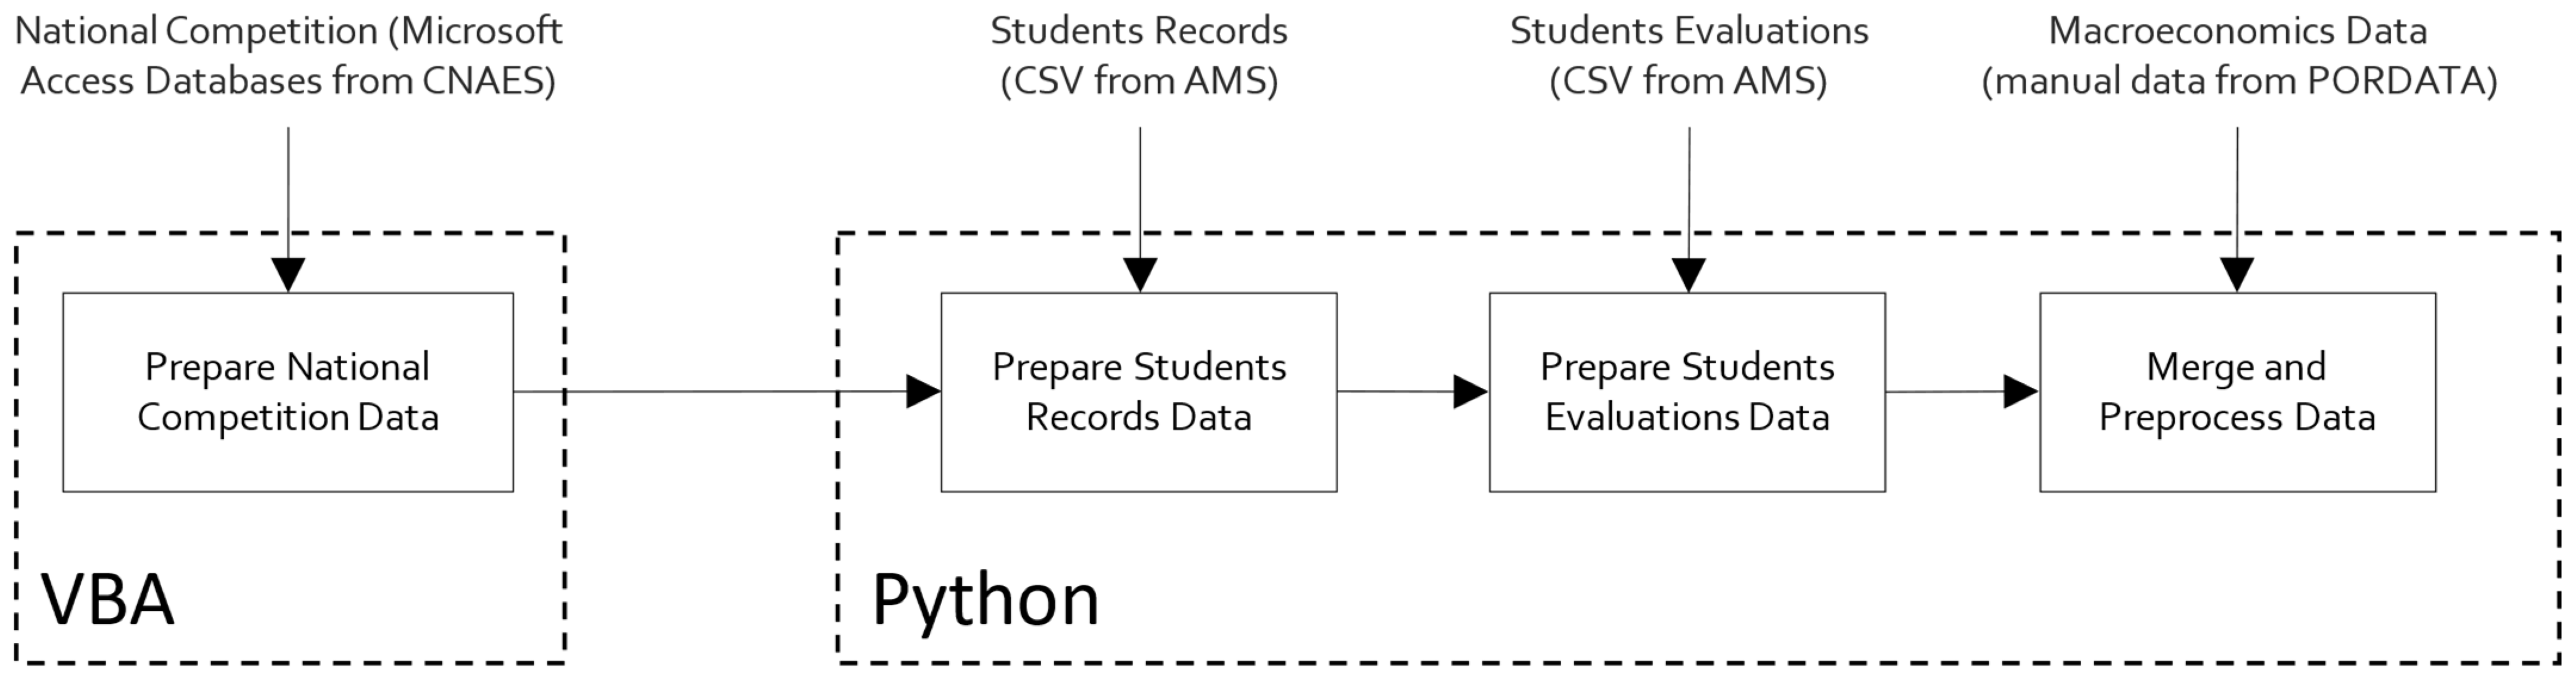
\includegraphics[width=\linewidth]{realinho2022-fig1}
    \nguon{Quy trình tạo bộ dữ liệu. Hình 1 gốc trong [1], CC BY 4.0.}
  \end{center}
  \textbf{Phân tích:} thống kê mô tả; kiểm tra mất cân bằng lớp và đa cộng tuyến (Pearson);
  \emph{Permutation Feature Importance} theo F1 với Random Forest, XGBoost, LightGBM, CatBoost.\par\medskip
  \textbf{Đạo đức dữ liệu:} đã ẩn danh, tuân thủ GDPR, được cán bộ bảo vệ dữ liệu của trường thẩm định [1].
}

% ================= COT 2 =================
\column{0.34}
\block{4. Kết quả chính}{
  \innerblock{Q1 -- Phân bố kết quả học tập}{
    \centering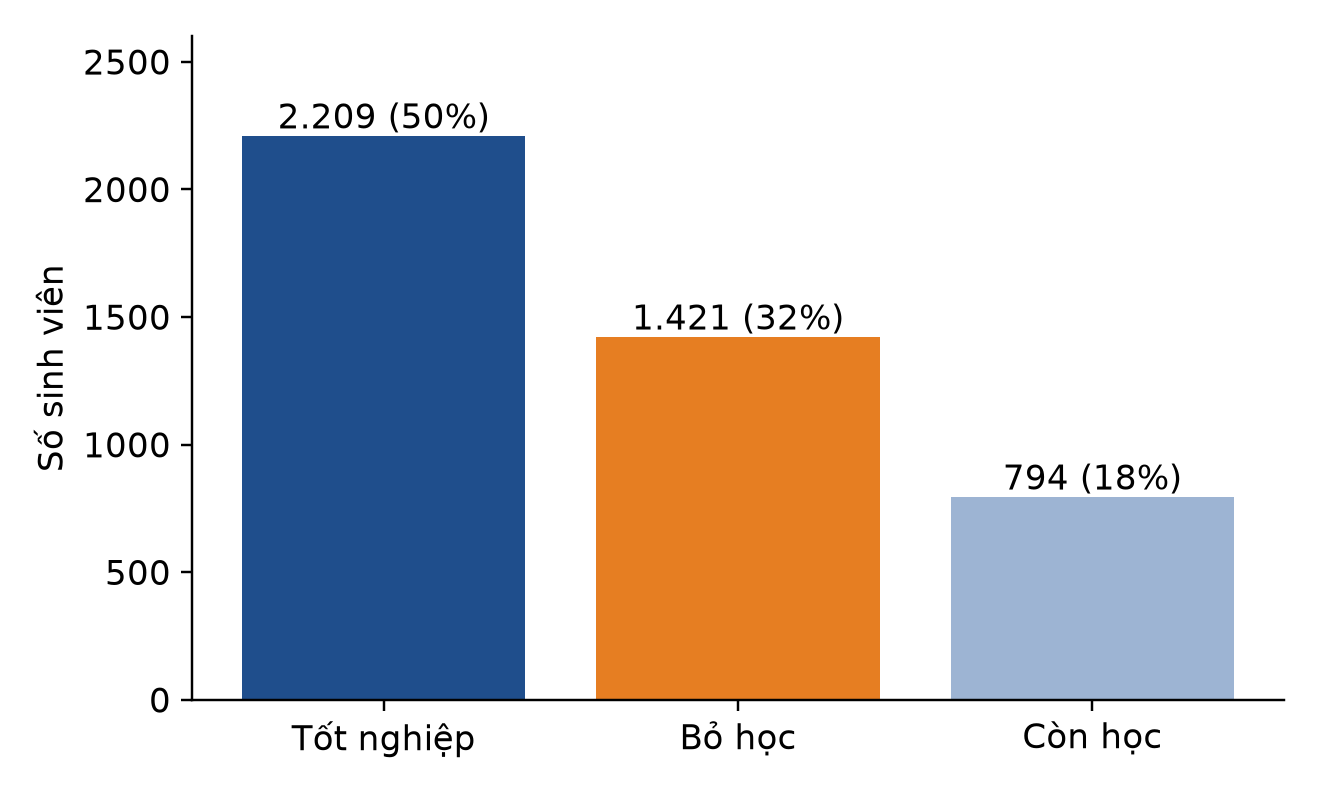
\includegraphics[width=0.82\linewidth]{rl_target}
    \nguon{Lớp mất cân bằng: 50\% tốt nghiệp, 32\% bỏ học, 18\% còn học.}
  }
  \par\bigskip
  \innerblock{Q2 -- Kết quả theo ngành học}{
    \centering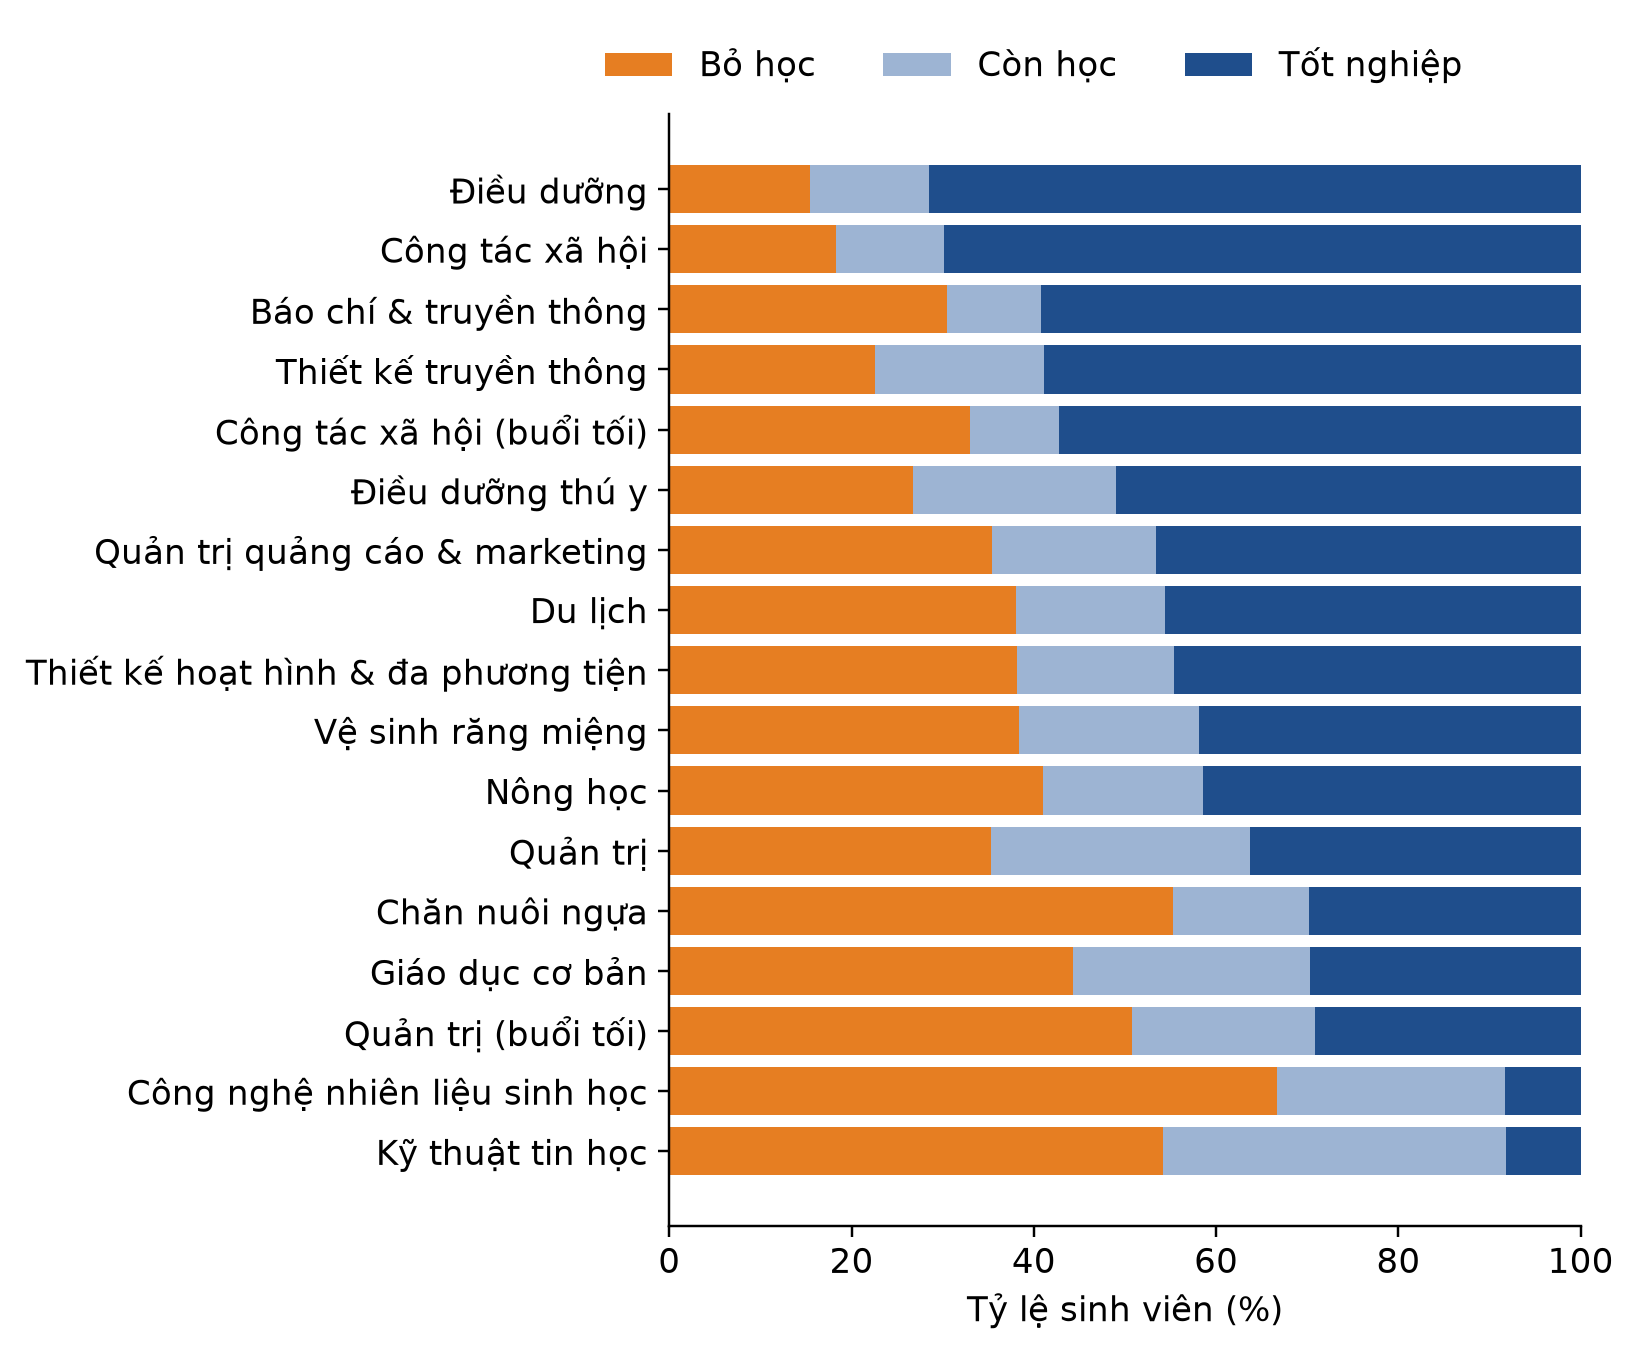
\includegraphics[width=\linewidth]{rl_by_course}
    \nguon{Điều dưỡng (72\%) và Công tác xã hội (70\%) tốt nghiệp đúng hạn nhiều nhất;
    Kỹ thuật tin học và Nhiên liệu sinh học chỉ 8\%.}
  }
  \par\bigskip
  \innerblock{Q2 -- Kết quả theo hoàn cảnh sinh viên}{
    \centering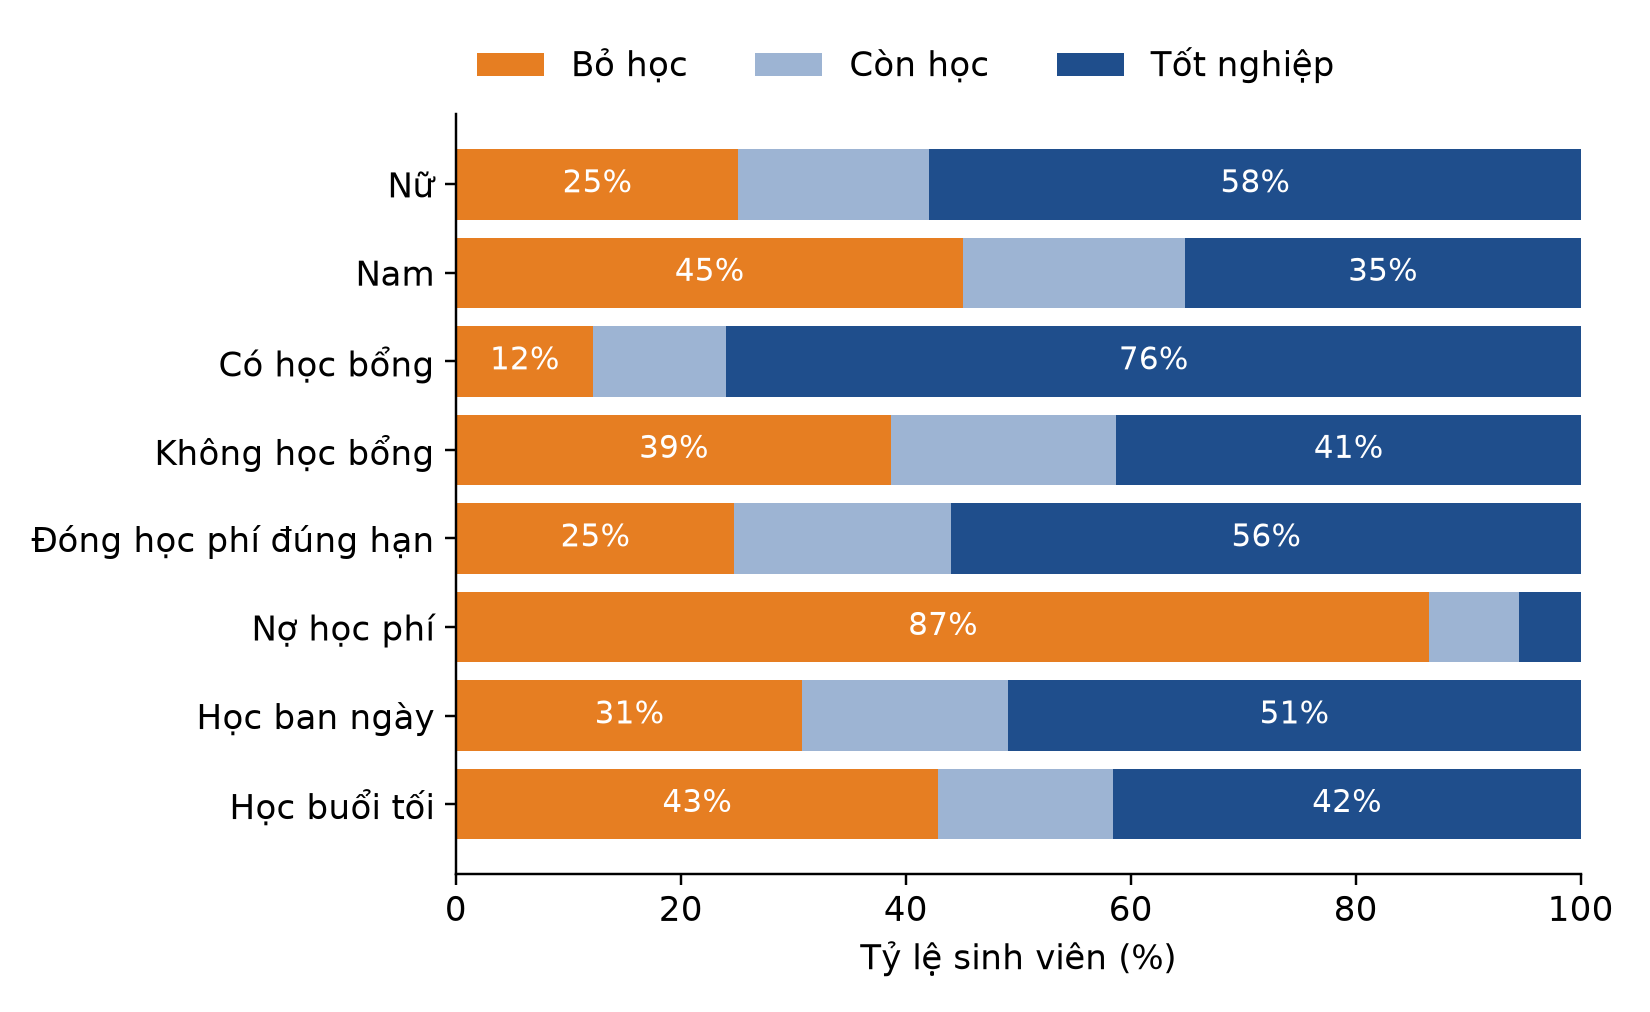
\includegraphics[width=\linewidth]{rl_by_group}
    \nguon{Nữ, có học bổng, đóng học phí đúng hạn và học ban ngày có tỷ lệ tốt nghiệp cao hơn.}
  }
  \nguon{Các biểu đồ trong khối 4 được vẽ lại từ dữ liệu gốc [2]; số liệu khớp với Hình 2 và Hình 3 của [1].}
}

% ================= COT 3 =================
\column{0.33}
\block{5. Phân tích \& thảo luận}{
  \innerblock{Q3 -- Đặc trưng quan trọng nhất}{
    \centering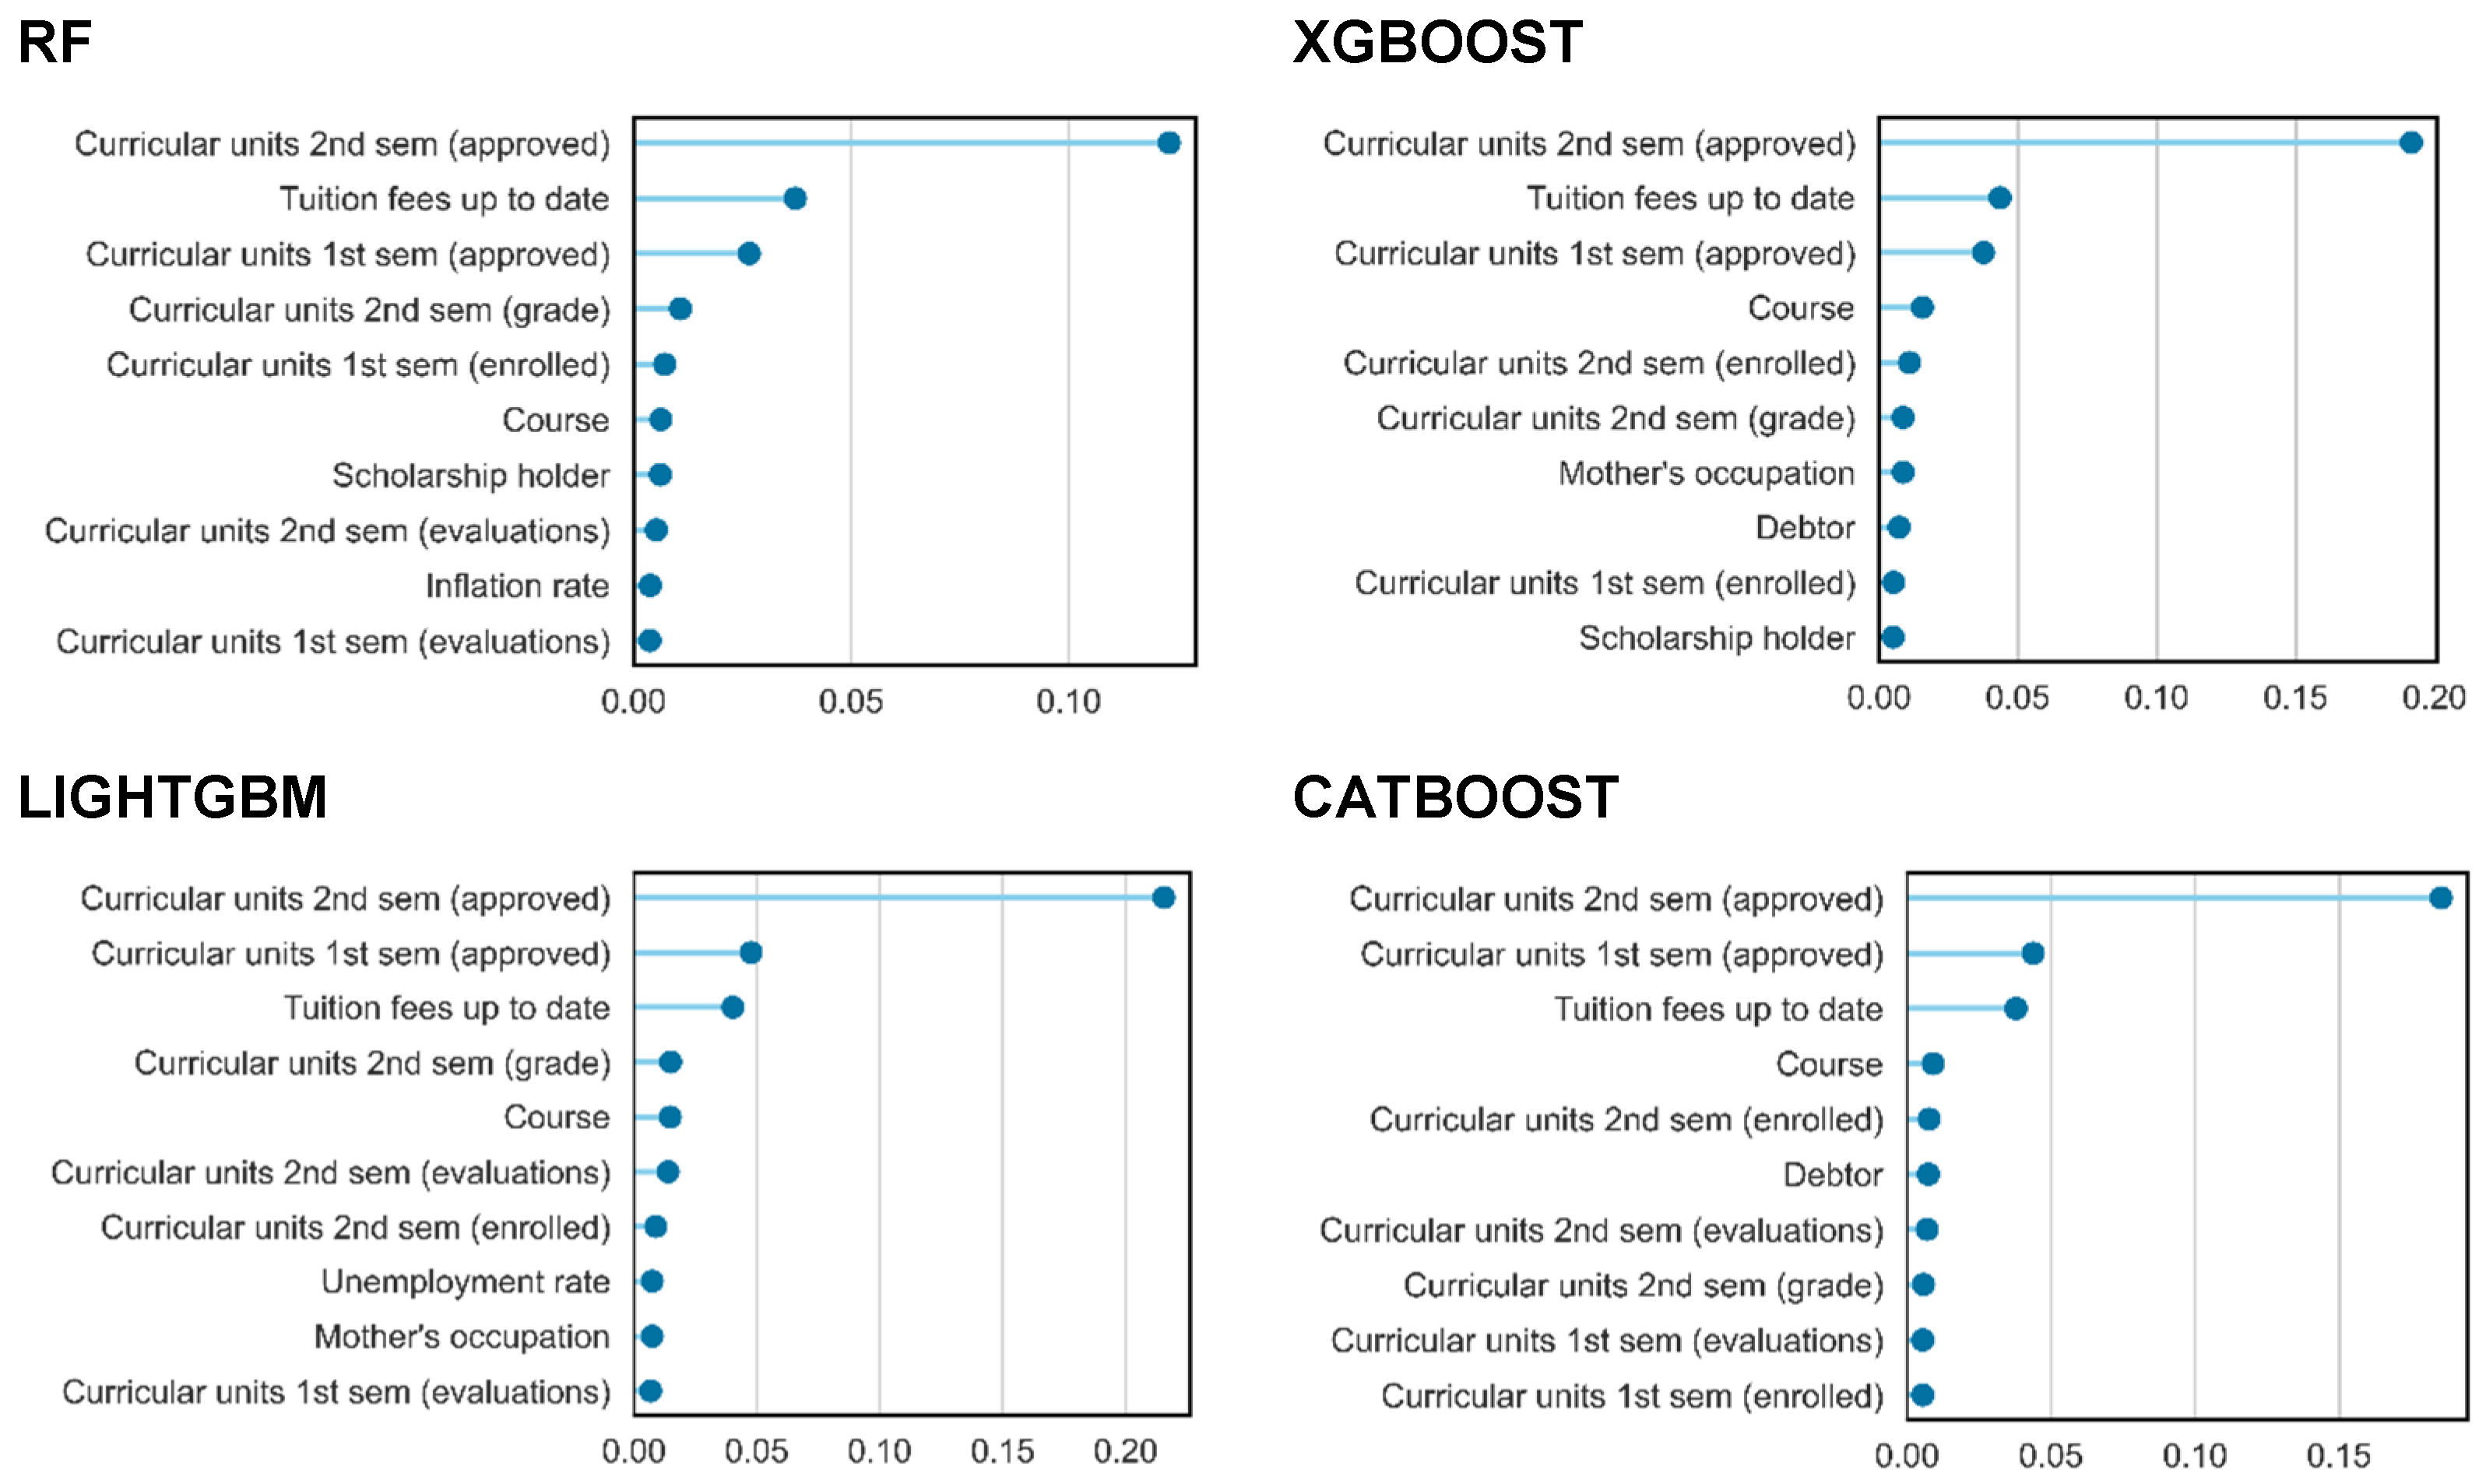
\includegraphics[width=\linewidth]{realinho2022-fig5}
    \nguon{Top 10 đặc trưng theo Permutation Feature Importance. Hình 5 gốc trong [1], CC BY 4.0.}
  }
  \par\medskip
  Năm đặc trưng quan trọng ở \textbf{cả bốn} thuật toán: số học phần đạt học kỳ 2 và học kỳ 1,
  điểm học kỳ 2, ngành học, và việc đóng học phí đúng hạn [1].
  \begin{center}
    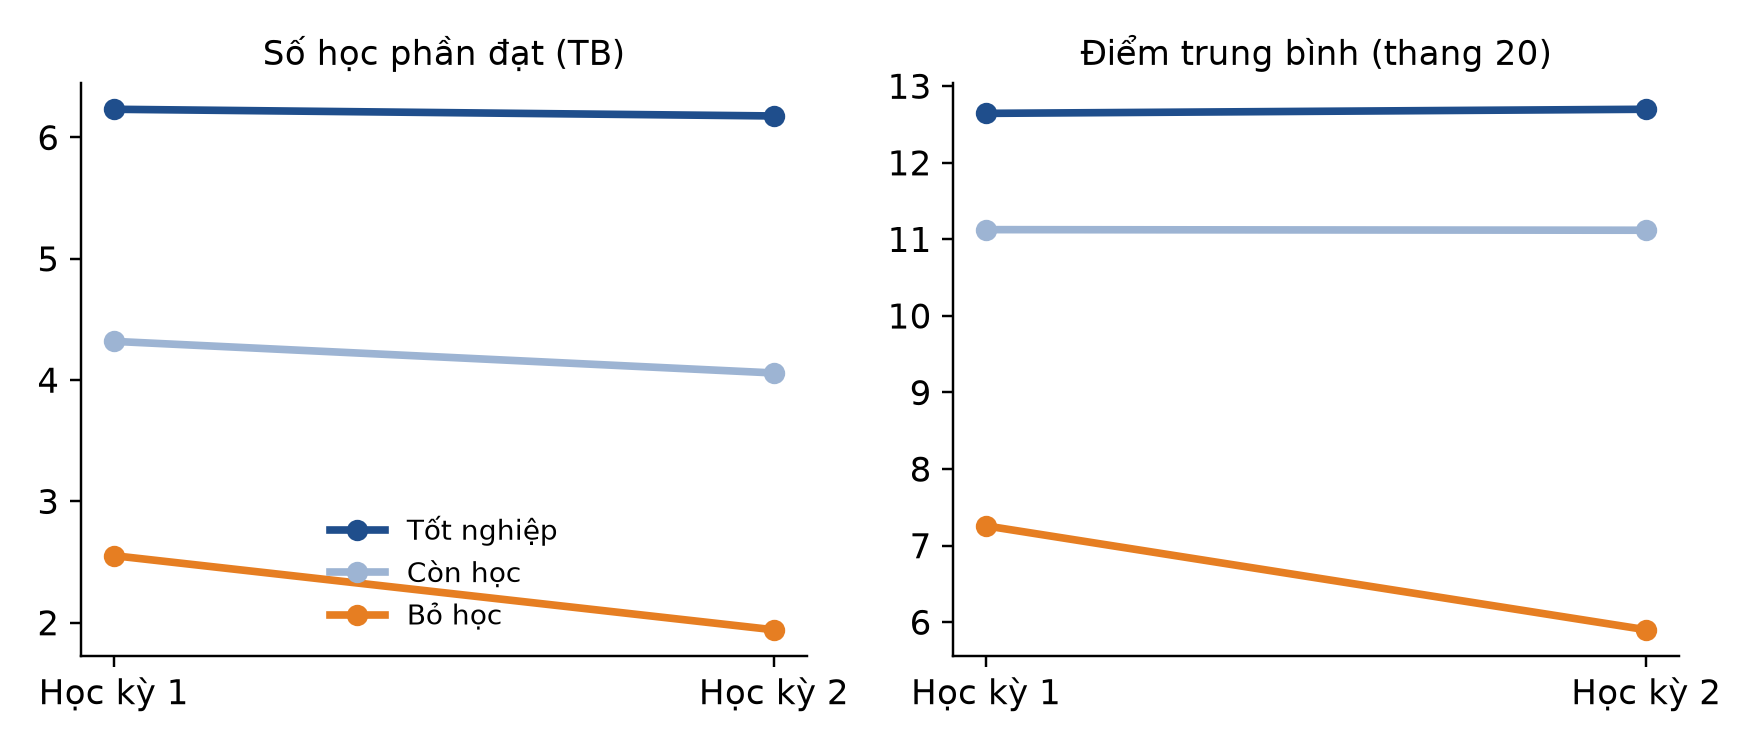
\includegraphics[width=0.85\linewidth]{rl_semester}
    \nguon{Nhóm bỏ học đạt ít học phần hơn hẳn ngay từ học kỳ 1 (vẽ lại từ [2]).}
  \end{center}
  Dữ liệu mất cân bằng nên cần SMOTE [3], ADASYN hoặc Balanced Random Forest; các biến cùng nhóm
  (học phần đạt học kỳ 1 và 2) có đa cộng tuyến cao [1].
}
\block{6. Kết luận \& hướng phát triển}{
  \begin{itemize}
    \item Bộ dữ liệu mở, sạch, phù hợp để so sánh thuật toán và đào tạo về học máy [1].
    \item Kết quả hai học kỳ đầu và tình trạng học phí là tín hiệu cảnh báo sớm mạnh nhất.
    \item \emph{Đề xuất của người trình bày:} áp dụng quy trình tương tự cho dữ liệu sinh viên
          Việt Nam đã ẩn danh, kết hợp kỹ thuật xử lý mất cân bằng.
  \end{itemize}
}
\block{Tài liệu tham khảo (IEEE)}{
  \footnotesize
  [1] V. Realinho, J. Machado, L. Baptista, M. V. Martins, ``Predicting Student Dropout and
      Academic Success,'' \emph{Data}, vol.~7, no.~11, p.~146, 2022, doi:10.3390/data7110146.\par
  [2] V. Realinho \emph{et al.}, ``Predict Students' Dropout and Academic Success'' [Dataset],
      UCI ML Repository, 2021, doi:10.24432/C5MC89. CC BY 4.0.\par
  [3] N. V. Chawla \emph{et al.}, ``SMOTE: Synthetic Minority Over-sampling Technique,''
      \emph{J. Artif. Intell. Res.}, vol.~16, pp.~321--357, 2002, doi:10.1613/jair.953.\par
  [4] A. Namoun, A. Alshanqiti, ``Predicting Student Performance Using Data Mining and Learning
      Analytics Techniques: A Systematic Literature Review,'' \emph{Appl. Sci.}, vol.~11, 237, 2021,
      doi:10.3390/app11010237.
}
\block{Liên hệ}{
  \begin{minipage}{0.62\linewidth}
    \textbf{Người trình bày:} Phạm Lê Trường Thịnh\par
    {\large email@student.ctu.edu.vn}\par\medskip
    Mọi số liệu và kết quả thuộc về nhóm tác giả của [1].\par\medskip
    Quét mã QR để đọc bài báo gốc.
  \end{minipage}\hfill
  \begin{minipage}{0.34\linewidth}\centering
    
\includegraphics[width=\linewidth]{qr-baibao}
  \end{minipage}
}
\end{columns}

\end{document}
